\chapter{Preliminaries}
\label{chap:prelim}
In this chapter we introduce the notation and definitions that will be used in the next chapters. Section~\ref{sec:prelim:foundations} formally defines event logs, traces and calendar windows. Section~\ref{sec:prelim:drift} formalizes concept drifts with drift points and drift modes. Section~\ref{sec:prelim:pca} describes scaling of features and PCA. Section~\ref{sec:prelim:clustering} presents the three clustering algorithms k-means, DBSCAN and SOMs used in our thesis.

\section{Foundations}
\label{sec:prelim:foundations}

An event log captures how a process was executed. In the traditional case-centric approach, each event in an event log belongs to exactly one case, relates to exactly one activity and has a timestamp. Case identifier, activity and timestamp are traditionally the required columns in event logs for process mining. Additional attributes like resources, durations, event attributes as well as case attributes allow additional analysis. In Section~\ref{sec:prelim:maths}, we introduce mathematical notation. Section~\ref{sec:prelim:logs} defines event logs, cases and traces, and Section~\ref{sec:prelim:windows} defines calendar windows.


\subsection{Mathematical Preliminaries}
\label{sec:prelim:maths}

% beginpenalty keeps each label on the same page as its first item
\noindent\emph{Sets:}
\begin{itemize}[beginpenalty=10000]
	\item A finite set $X = \{a_1, a_2, ..., a_n\}$ is a finite collection of objects.
	\item The power set $\mathcal{P}(X)$ of $X$ denotes the set of all subsets of $X$.
	\item $\N$ is the set of natural numbers, $\Z$ is the set of integers, $\R$ the set of real numbers and $\N_0 = \N \cup \Set{0}$ is the set of natural numbers including $0$.
\end{itemize}

\noindent\emph{Functions:}
\begin{itemize}[beginpenalty=10000]
	\item A function $f$ from a set $X$ to a set $Y$ maps each element of its domain $\dom(f) \subseteq X$ to exactly one element of $Y$.
	\item $X \pto Y$ is the set of all functions from $X$ to $Y$, which we call partial functions.
	\item $X \to Y$ is the set of all total functions from $X$ to $Y$, i.e., of all $f \in X \pto Y$ with $\dom(f) = X$.
	\item For a set $Q$, $f{\restriction}_Q$ is the restriction of $f$ to $Q$ with $\dom(f{\restriction}_Q) = \dom(f) \cap Q$ and $f{\restriction}_Q(x) = f(x)$ for all $x \in \dom(f{\restriction}_Q)$.
\end{itemize}

\noindent\emph{Multisets:}
\begin{itemize}[beginpenalty=10000]
	\item A multiset is a set where an element can occur multiple times.
	\item $\mathcal{B}(A) = A \to \N_0$ is the set of all multisets over a set $A$.
	\item For $X \in \mathcal{B}(A)$ and $a \in A$, $X(a)$ is the multiplicity of $a$ in $X$.
	\item We write multisets as $X = [x^3, y^2, z]$, meaning $X(x) = 3$, $X(y) = 2$ and $X(z) = 1$.
	\item $[\,]$ is the empty multiset, and $\abs{X} = \sum_{a \in A} X(a)$ is the size of a finite multiset $X$.
\end{itemize}

\noindent\emph{Sequences:}
\begin{itemize}[beginpenalty=10000]
	\item A sequence is an ordered collection of objects in which an object can occur multiple times.
	\item $X^*$ is the set of all finite sequences over a set $X$, and $\seq{}$ is the empty sequence.
	\item A sequence $\sigma = \seq{a_1, \dots, a_n} \in X^*$ has the length $\abs{\sigma} = n$, and $\sigma(i) = a_i$ is its $i$-th element for $1 \le i \le n$.
	\item For $0 \le k \le n$, $\mathit{prefix}_k(\sigma) = \seq{a_1, \dots, a_k}$ is the prefix of length~$k$.
	\item $\partial_{\mathit{set}}(\sigma) = \Set{a_1, \dots, a_n}$ turns $\sigma$ into a set.
	\item $\partial_{\mathit{multiset}}(\sigma) = [a_1, \dots, a_n]$ turns $\sigma$ into a multiset, e.g., $\partial_{\mathit{multiset}}(\seq{a, b, b}) = [a, b^2]$.
	\item $\mathit{df}(\sigma) = \MultiSet{(a_i, a_{i+1}) \given 1 \le i < n} \in \mathcal{B}(X \times X)$ is the multiset of directly-follows pairs of $\sigma$, e.g., $\mathit{df}(\seq{a, b, b, c}) = [(a, b), (b, b), (b, c)]$.
\end{itemize}


\subsection{Event Logs, Cases and Traces}
\label{sec:prelim:logs}
We define event logs as a set of events using an attribute function. In this notation, each event is uniquely identifiable even if two events have the same attribute values.

\medskip
\noindent\emph{Universes:}
\begin{itemize}[beginpenalty=10000]
	\item $\U{ev}$ is the universe of events.
	\item $\U{case}$ is the universe of case identifiers, $\U{act}$ is the universe of activities and $\U{res}$ is the universe of resources.
	\item $\U{time}$ is the universe of timestamps.
	\item $\U{att}$ is the universe of attribute names with $\Set{\mathit{case}, \mathit{act}, \mathit{time}, \mathit{res}} \subseteq \U{att}$.
	\item $\U{val}$ is the universe of attribute values with $\U{case} \cup \U{act} \cup \U{time} \cup \U{res} \subseteq \U{val}$.
	\item $\U{map} = \U{att} \pto \U{val}$ is the universe of attribute value mappings.
\end{itemize}

\begin{definition}[Event Log]
	\label{def:prelim:event_log}
	An event log is a tuple $L = (E, \pi, \preceq)$ with
	\begin{itemize}
		\item a finite set of events $E \subseteq \U{ev}$,
		\item an attribute function $\pi \in E \to \U{map}$ such that for each event $e \in E$:
		      \begin{itemize}
			      \item $\Set{\mathit{case}, \mathit{act}, \mathit{time}} \subseteq \dom(\pi(e))$ with $\pi(e)(\mathit{case}) \in \U{case}$, $\pi(e)(\mathit{act}) \in \U{act}$ and $\pi(e)(\mathit{time}) \in \U{time}$,
			      \item $\mathit{res} \in \dom(\pi(e)) \Rightarrow \pi(e)(\mathit{res}) \in \U{res}$,
		      \end{itemize}
		\item a total order $\preceq$ on $E$ that respects the timestamps, i.e., $e \preceq e'$ for all $e, e' \in E$ with $\pi(e)(\mathit{time}) < \pi(e')(\mathit{time})$.
	\end{itemize}
	Furthermore:
	\begin{itemize}
		\item For $e \in E$ and $n \in \dom(\pi(e))$, $\pi_n(e) = \pi(e)(n)$ is the value of attribute $n$ of $e$, e.g., $\pi_{\mathit{act}}(e)$ is the activity of $e$.
		\item An attribute name $n \in \U{att} \setminus \Set{\mathit{case}, \mathit{act}, \mathit{time}, \mathit{res}}$ is a case attribute of $L$ if all events of a case have the same value for $n$, i.e., $\pi(e){\restriction}_{\Set{n}} = \pi(e'){\restriction}_{\Set{n}}$ for all $e, e' \in E$ with $\pi_{\mathit{case}}(e) = \pi_{\mathit{case}}(e')$.
	\end{itemize}
\end{definition}

\begin{definition}[Case, Trace and Prefix]
	\label{def:prelim:trace}
	Let $L = (E, \pi, \preceq)$ be an event log.
	\begin{itemize}
		\item $C_L = \Set{\pi_{\mathit{case}}(e) \given e \in E}$ is the set of cases of $L$.
		\item For a case $c \in C_L$, $E_L(c) = \Set{e \in E \given \pi_{\mathit{case}}(e) = c}$ is the set of its events.
		\item Let $e_1, \dots, e_n$ be the events of a case $c \in C_L$ in the order $\preceq$, i.e., $\Set{e_1, \dots, e_n} = E_L(c)$, $n = \abs{E_L(c)}$ and $e_i \preceq e_{i+1}$ for $1 \le i < n$. Then
		      \begin{itemize}
			      \item $\mathit{trace}_L(c) = \seq{\pi_{\mathit{act}}(e_1), \dots, \pi_{\mathit{act}}(e_n)} \in \U{act}^*$ is the trace of $c$,
			      \item $\mathit{start}_L(c) = \pi_{\mathit{time}}(e_1)$ is the start of $c$,
			      \item $\mathit{end}_L(c) = \pi_{\mathit{time}}(e_n)$ is the end of $c$ and
			      \item $\mathit{prefix}_L(e_k) = \mathit{prefix}_k(\mathit{trace}_L(c))$ is the prefix of the event $e_k$ for $1 \le k \le n$.
		      \end{itemize}
	\end{itemize}
\end{definition}

\begin{table}[tb]
	\centering
	\caption[Example event log table]{%
		Event log $L_1$ with three cases and eleven events. Each row is an event with its attributes, and the second header row gives the attribute names. The activities are $a$, $b$, $c$ and $d$. The timestamp is the completion time of an event, and the duration is its processing time in minutes. The amount in euros is a case attribute.}
	\label{tab:prelim:example_log}
	\begin{tabular}{@{}cccllrr@{}}
		\toprule
		Event    & Case            & Activity       & Timestamp        & Resource       & Duration            & Amount            \\
		         & $\mathit{case}$ & $\mathit{act}$ & $\mathit{time}$  & $\mathit{res}$ & $\mathit{duration}$ & $\mathit{amount}$ \\
		\midrule
		$e_1$    & 1               & $a$            & 2020-03-02 08:15 & Anna           & 15                  & 5000              \\
		$e_2$    & 1               & $b$            & 2020-03-02 10:40 & Ben            & 45                  & 5000              \\
		$e_3$    & 1               & $c$            & 2020-03-02 15:05 & Clara          & 25                  & 5000              \\
		$e_4$    & 1               & $d$            & 2020-03-03 09:30 & Anna           & 5                   & 5000              \\
		\addlinespace
		$e_5$    & 2               & $a$            & 2020-03-02 09:00 & Anna           & 10                  & 1200              \\
		$e_6$    & 2               & $c$            & 2020-03-02 13:20 & Clara          & 30                  & 1200              \\
		$e_7$    & 2               & $d$            & 2020-03-02 16:45 & Ben            & 10                  & 1200              \\
		\addlinespace
		$e_8$    & 3               & $a$            & 2020-03-02 14:10 & Anna           & 20                  & 8000              \\
		$e_9$    & 3               & $b$            & 2020-03-03 08:50 & Ben            & 40                  & 8000              \\
		$e_{10}$ & 3               & $b$            & 2020-03-03 11:30 & Ben            & 55                  & 8000              \\
		$e_{11}$ & 3               & $c$            & 2020-03-03 16:00 & Clara          & 20                  & 8000              \\
		\bottomrule
	\end{tabular}
\end{table}

\begin{example}
	\label{ex:prelim:event_log}
	Table~\ref{tab:prelim:example_log} shows the event log $L_1 = (E, \pi, \preceq)$ with the events $E = \Set{e_1, \dots, e_{11}}$.

	\begin{itemize}
		\item $\U{ev} = E = \Set{e_1, \dots, e_{11}}$.
		
		\item $\U{case} = \Set{1, 2, 3}$, $\U{act} = \Set{a, b, c, d}$ and $\U{res} = \Set{\text{Anna}, \text{Ben}, \text{Clara}}$.
		
		\item $\U{att} = \Set{\mathit{case}, \mathit{act}, \mathit{time}, \mathit{res}, \mathit{duration}, \mathit{amount}}$.
		
		\item $\U{val} = \R \cup \Set{a, b, c, d, \text{Anna}, \text{Ben}, \text{Clara}} \cup \U{time} \supseteq \U{case} \cup \U{act} \cup \U{time} \cup \U{res}$. The case IDs, durations and amounts are real numbers and therefore also in $\U{val}$.
		
		\item $\U{map} = \U{att} \pto \U{val}$ is the set of all partial functions from these six attribute names to values, e.g., $\Set{(\mathit{act}, b)} \in \U{map}$ and $\emptyset \in \U{map}$.
		
		\item $\pi \in E \to \U{map}$ maps each event to the attribute value mapping of its row in Table~\ref{tab:prelim:example_log}, e.g.,
			\[
		\begin{aligned}
			\pi(e_9) = \{ & (\mathit{case}, 3), (\mathit{act}, b), (\mathit{time}, \text{2020-03-03 08:50}), \\
			              & (\mathit{res}, \text{Ben}), (\mathit{duration}, 40), (\mathit{amount}, 8000)\}.
		\end{aligned}
			\]
		\item For all attribute names $n \in \U{att}$, the values of $e_9$ are $\pi_{\mathit{case}}(e_9) = 3$, $\pi_{\mathit{act}}(e_9) = b$, $\pi_{\mathit{time}}(e_9) = \text{2020-03-03 08:50}$, $\pi_{\mathit{res}}(e_9) = \text{Ben}$, $\pi_{\mathit{duration}}(e_9) = 40$ and $\pi_{\mathit{amount}}(e_9) = 8000$.
		
		\item $\mathit{amount}$ is a case attribute, since all events of a case have the same amount, e.g., $\pi(e){\restriction}_{\Set{\mathit{amount}}} = \Set{(\mathit{amount}, 8000)}$ for the four events $e$ of case~3.

		\item \emph{Cases and traces:} $L_1$ has the cases $C_{L_1} = \Set{1, 2, 3}$. Case~3 has the events $e_8 \preceq e_9 \preceq e_{10} \preceq e_{11}$ and thus the trace $\mathit{trace}_{L_1}(3) = \seq{a, b, b, c}$. It starts at \mbox{2020-03-02 14:10} and ends at \mbox{2020-03-03 16:00}. The prefix of $e_{10}$ is $\sigma = \mathit{prefix}_{L_1}(e_{10}) = \seq{a, b, b}$ with $\partial_{\mathit{multiset}}(\sigma) = [a, b^2]$ and $\mathit{df}(\sigma) = [(a, b), (b, b)]$.
	\end{itemize}



	
\end{example}

\subsection{Calendar Windows}
\label{sec:prelim:windows}
We use calendar windows, i.e., time intervals of fixed length that start at calendar boundaries such as midnight. Thus, the window boundaries only depend on the origin and the window length, and not on the first event of the event log. To compute with timestamps, we treat them as real numbers, e.g., the seconds since a fixed point in time.

\begin{definition}[Calendar Window]
	\label{def:prelim:windows}
	Let $o \in \U{time}$ be an origin and $\Delta \in \R$ with $\Delta > 0$ a window length.
	\begin{itemize}
		\item For $k \in \Z$, $w_k = [o + k\Delta, o + (k+1)\Delta)$ is the $k$-th calendar window.
		\item A timestamp $t \in \U{time}$ lies in the window $w_k$ if $t \in w_k$, i.e., $k = \lfloor (t - o) / \Delta \rfloor$.
	\end{itemize}
\end{definition}

\begin{figure}[tb]
	\centering
	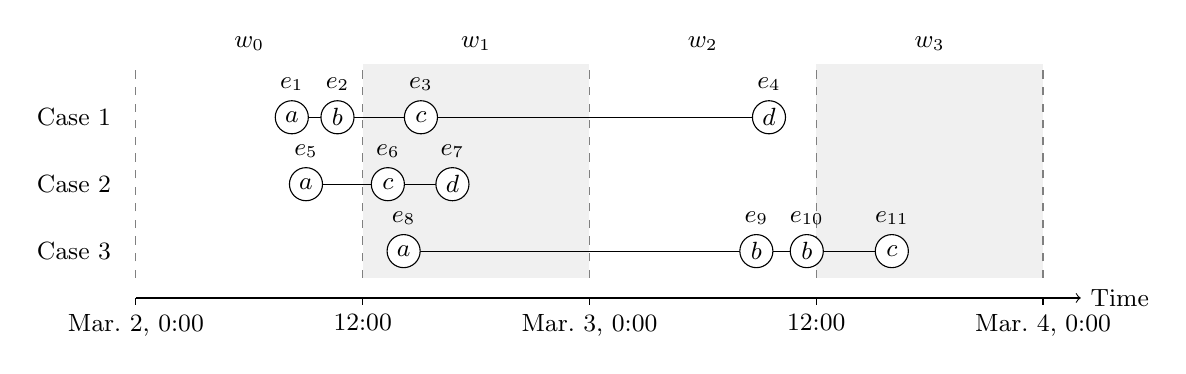
\begin{tikzpicture}[x=0.24cm, y=0.85cm, font=\small]
		% alternate shading of the calendar windows
		\fill[black!6] (12, -0.4) rectangle (24, 2.8);
		\fill[black!6] (36, -0.4) rectangle (48, 2.8);
		% window boundaries and names
		\foreach \h in {0, 12, 24, 36, 48}
			\draw[dashed, black!50] (\h, -0.4) -- (\h, 2.8);
		\foreach \h/\w in {6/0, 18/1, 30/2, 42/3}
			\node at (\h, 3.1) {$w_{\w}$};
		% cases
		\node[anchor=east] at (-0.8, 2) {Case 1};
		\node[anchor=east] at (-0.8, 1) {Case 2};
		\node[anchor=east] at (-0.8, 0) {Case 3};
		% events of a case in their order, one unit on the x-axis is one hour from 2020-03-02 0:00
		\draw (8.25, 2) -- (10.667, 2) -- (15.083, 2) -- (33.5, 2);
		\draw (9, 1) -- (13.333, 1) -- (16.75, 1);
		\draw (14.167, 0) -- (32.833, 0) -- (35.5, 0) -- (40, 0);
		% events with their activity
		\foreach \h/\y/\act/\e in {8.25/2/a/1, 10.667/2/b/2, 15.083/2/c/3, 33.5/2/d/4, 9/1/a/5, 13.333/1/c/6, 16.75/1/d/7, 14.167/0/a/8, 32.833/0/b/9, 35.5/0/b/10, 40/0/c/11} {
			\node[circle, draw, fill=white, inner sep=0pt, minimum size=0.42cm] at (\h, \y) {$\act$};
			\node[above=0.21cm] at (\h, \y) {$e_{\e}$};
		}
		% time axis
		\draw[->] (0, -0.7) -- (50, -0.7) node[right] {Time};
		\foreach \h/\lab in {0/{Mar.~2, 0:00}, 12/{12:00}, 24/{Mar.~3, 0:00}, 36/{12:00}, 48/{Mar.~4, 0:00}}
			\draw (\h, -0.7) -- (\h, -0.8) node[below] {\lab};
	\end{tikzpicture}
	\caption[Example event log with calendar windows]{%
		Event log $L_1$ from Table~\ref{tab:prelim:example_log} on a time axis. Each row shows the events of a case in their order, and each circle is an event with its activity. Dashed lines separate the calendar windows $w_0$ to $w_3$ with the origin 2020-03-02 0:00 and the length $\Delta = 12$~hours. A case often spans several windows, and a window contains events of several cases.}
	\label{fig:prelim:windows}
\end{figure}

\begin{example}
	\label{ex:prelim:windows}
	Figure~\ref{fig:prelim:windows} shows $L_1$ from Example~\ref{ex:prelim:event_log} with the window length $\Delta = 12$~hours and the origin $o$ = \mbox{2020-03-02 0:00}.
	\begin{itemize}
		\item For $k = 1$, the window is $w_1 = [\text{2020-03-02 12:00}, \text{2020-03-03 0:00})$.

		\item The timestamp $t$ = \mbox{2020-03-02 15:05} of $e_3$ lies in $w_1$.

		\item The timestamps of $e_3$, $e_6$, $e_7$ and $e_8$ lie in $w_1$, so $w_1$ contains events of all three cases.

		\item A case often spans several windows, e.g., the timestamps of case~3 lie in $w_1$, $w_2$ and $w_3$.
	\end{itemize}
\end{example}

\section{Concept Drift}
\label{sec:prelim:drift}
In this section, we formalize concept drifts. The building block of a concept drift is the process change, which replaces one process version by another. 

A concept drift is a situation in which a process changes. According to \textcite{kraus2026characterization}, an event log with a drift then contains data from different process versions. They describe a process version by the process model that governs its execution. We use a broader notion. Besides the control-flow, a process version also determines which resources execute which activities, how long activities take and how long a case waits between two events. It also determines how many cases arrive and which values their case attributes take. The drift type describes in which of these properties two versions differ (Section~\ref{sec:intro_ssec:motiv}).

\begin{definition}[Process Change]
	\label{def:prelim:change}
	Let $V$ be a set of process versions. A process change is a tuple $(v, v', t_s, t_e) \in V \times V \times \U{time} \times \U{time}$ with $v \neq v'$ and $t_s \le t_e$ such that
	\begin{itemize}
		\item before $t_s$, the process behaves according to version $v$,
		\item from $t_e$ on, the process behaves according to version $v'$ and
		\item between $t_s$ and $t_e$, the process changes gradually from $v$ to $v'$.
	\end{itemize}
	$t_s$ and $t_e$ are the drift points of the change. The change is sudden if $t_s = t_e$, and gradual otherwise.
\end{definition}

In a gradual change, both versions coexist for some time, and the old version is discontinued gradually. We assume that the share of behavior that follows $v'$ grows linearly between $t_s$ and $t_e$.

\begin{definition}[Concept Drift, Drift Mode]
	\label{def:prelim:drift}
	Let $V$ be a set of process versions. A concept drift is a sequence
	\[
		\delta = \seq{(v_1, v_2, s_1, t_1), (v_2, v_3, s_2, t_2), \dots, (v_m, v_{m+1}, s_m, t_m)}
	\]
	of $m \ge 1$ process changes with $t_i \le s_{i+1}$ for $1 \le i < m$. The drift points of $\delta$ are the drift points of its changes. The drift mode of $\delta$ is
	\begin{itemize}
		\item \emph{sudden} if $m = 1$ and $s_1 = t_1$,
		\item \emph{gradual} if $m = 1$ and $s_1 < t_1$,
		\item \emph{recurring} if $m \ge 2$ and a version occurs more than once, i.e., $v_i = v_j$ for some $1 \le i < j \le m + 1$,
		\item \emph{incremental} if $m \ge 2$, the versions $v_1, \dots, v_{m+1}$ are pairwise different and each change alters the process only slightly, where all changes follow the same initiative.
	\end{itemize}
\end{definition}

The four drift modes originate from the taxonomy of \textcite{bose2011handling}, and \textcite{kraus2026characterization} call them drift types. We call them drift modes instead and reserve the term drift type for what changes. In this thesis we will focus on sudden and gradual drifts. Figure~\ref{fig:prelim:drift_modes} shows the four drift modes.

\begin{figure}[tb]
	\centering
	\definecolor{versionA}{RGB}{0,114,178}
	\definecolor{versionB}{RGB}{86,180,233}
	\definecolor{versionC}{RGB}{0,158,115}
	\definecolor{versionD}{RGB}{230,159,0}
	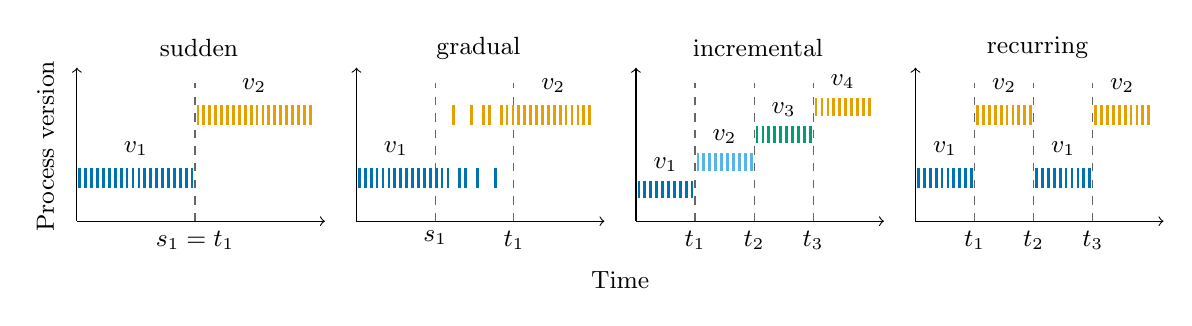
\begin{tikzpicture}[font=\small, case/.style={line width=1pt}]
		% axis labels shared by the four panels
		\node[rotate=90] at (-0.4, 0.95) {Process version};
		\node at (6.9, -0.75) {Time};
		% sudden: one change at 1.5
		\begin{scope}
			\draw[->] (0, 0) -- (3.15, 0);
			\draw[->] (0, 0) -- (0, 1.95);
			\node at (1.55, 2.2) {sudden};
			\draw[dashed, black!60] (1.5, 0) -- (1.5, 1.75);
			\node[below] at (1.5, 0) {$s_1 = t_1$};
			\foreach \x in {0.0375, 0.1125, 0.1875, 0.2625, 0.3375, 0.4125, 0.4875, 0.5625, 0.6375, 0.7125, 0.7875, 0.8625, 0.9375, 1.0125, 1.0875, 1.1625, 1.2375, 1.3125, 1.3875, 1.4625}
				\draw[case, versionA] (\x, 0.42) -- (\x, 0.68);
			\foreach \x in {1.5375, 1.6125, 1.6875, 1.7625, 1.8375, 1.9125, 1.9875, 2.0625, 2.1375, 2.2125, 2.2875, 2.3625, 2.4375, 2.5125, 2.5875, 2.6625, 2.7375, 2.8125, 2.8875, 2.9625}
				\draw[case, versionD] (\x, 1.22) -- (\x, 1.48);
			\node at (0.75, 0.92) {$v_1$};
			\node at (2.25, 1.72) {$v_2$};
		\end{scope}
		% gradual: change between 1.0 and 2.0
		\begin{scope}[xshift=3.55cm]
			\draw[->] (0, 0) -- (3.15, 0);
			\draw[->] (0, 0) -- (0, 1.95);
			\node at (1.55, 2.2) {gradual};
			\draw[dashed, black!60] (1, 0) -- (1, 1.75);
			\draw[dashed, black!60] (2, 0) -- (2, 1.75);
			\node[below] at (1, 0) {$s_1$};
			\node[below] at (2, 0) {$t_1$};
			\foreach \x in {0.0375, 0.1125, 0.1875, 0.2625, 0.3375, 0.4125, 0.4875, 0.5625, 0.6375, 0.7125, 0.7875, 0.8625, 0.9375, 1.0125, 1.0875, 1.1625, 1.3125, 1.3875, 1.5375, 1.7625}
				\draw[case, versionA] (\x, 0.42) -- (\x, 0.68);
			\foreach \x in {1.2375, 1.4625, 1.6125, 1.6875, 1.8375, 1.9125, 1.9875, 2.0625, 2.1375, 2.2125, 2.2875, 2.3625, 2.4375, 2.5125, 2.5875, 2.6625, 2.7375, 2.8125, 2.8875, 2.9625}
				\draw[case, versionD] (\x, 1.22) -- (\x, 1.48);
			\node at (0.5, 0.92) {$v_1$};
			\node at (2.5, 1.72) {$v_2$};
		\end{scope}
		% incremental: three small changes at 0.75, 1.5 and 2.25
		\begin{scope}[xshift=7.1cm]
			\draw[->] (0, 0) -- (3.15, 0);
			\draw[->] (0, 0) -- (0, 1.95);
			\node at (1.55, 2.2) {incremental};
			\foreach \x/\idx in {0.75/1, 1.5/2, 2.25/3} {
				\draw[dashed, black!60] (\x, 0) -- (\x, 1.75);
				\node[below] at (\x, 0) {$t_{\idx}$};
			}
			\foreach \x in {0.0375, 0.1125, 0.1875, 0.2625, 0.3375, 0.4125, 0.4875, 0.5625, 0.6375, 0.7125}
				\draw[case, versionA] (\x, 0.29) -- (\x, 0.51);
			\foreach \x in {0.7875, 0.8625, 0.9375, 1.0125, 1.0875, 1.1625, 1.2375, 1.3125, 1.3875, 1.4625}
				\draw[case, versionB] (\x, 0.64) -- (\x, 0.86);
			\foreach \x in {1.5375, 1.6125, 1.6875, 1.7625, 1.8375, 1.9125, 1.9875, 2.0625, 2.1375, 2.2125}
				\draw[case, versionC] (\x, 0.99) -- (\x, 1.21);
			\foreach \x in {2.2875, 2.3625, 2.4375, 2.5125, 2.5875, 2.6625, 2.7375, 2.8125, 2.8875, 2.9625}
				\draw[case, versionD] (\x, 1.34) -- (\x, 1.56);
			\node at (0.375, 0.72) {$v_1$};
			\node at (1.125, 1.07) {$v_2$};
			\node at (1.875, 1.42) {$v_3$};
			\node at (2.625, 1.77) {$v_4$};
		\end{scope}
		% recurring: v1 and v2 alternate at 0.75, 1.5 and 2.25
		\begin{scope}[xshift=10.65cm]
			\draw[->] (0, 0) -- (3.15, 0);
			\draw[->] (0, 0) -- (0, 1.95);
			\node at (1.55, 2.2) {recurring};
			\foreach \x/\idx in {0.75/1, 1.5/2, 2.25/3} {
				\draw[dashed, black!60] (\x, 0) -- (\x, 1.75);
				\node[below] at (\x, 0) {$t_{\idx}$};
			}
			\foreach \x in {0.0375, 0.1125, 0.1875, 0.2625, 0.3375, 0.4125, 0.4875, 0.5625, 0.6375, 0.7125, 1.5375, 1.6125, 1.6875, 1.7625, 1.8375, 1.9125, 1.9875, 2.0625, 2.1375, 2.2125}
				\draw[case, versionA] (\x, 0.42) -- (\x, 0.68);
			\foreach \x in {0.7875, 0.8625, 0.9375, 1.0125, 1.0875, 1.1625, 1.2375, 1.3125, 1.3875, 1.4625, 2.2875, 2.3625, 2.4375, 2.5125, 2.5875, 2.6625, 2.7375, 2.8125, 2.8875, 2.9625}
				\draw[case, versionD] (\x, 1.22) -- (\x, 1.48);
			\node at (0.375, 0.92) {$v_1$};
			\node at (1.125, 1.72) {$v_2$};
			\node at (1.875, 0.92) {$v_1$};
			\node at (2.625, 1.72) {$v_2$};
		\end{scope}
	\end{tikzpicture}
	\caption[The four drift modes]{%
		The four drift modes. Each tick is a case, and its height and color show the process version it follows. Dashed lines mark the drift points. A sudden change replaces $v_1$ by $v_2$ at one point in time. In a gradual change, more and more cases follow $v_2$ between $s_1$ and $t_1$. An incremental drift leads from $v_1$ to $v_4$ in small steps, and a recurring drift returns to earlier versions. The changes of the incremental and the recurring drift are sudden here, i.e., $s_i = t_i$.}
	\label{fig:prelim:drift_modes}
\end{figure}

\begin{example}
	\label{ex:prelim:drift}
	The following drift illustrates Definitions~\ref{def:prelim:change} and~\ref{def:prelim:drift}.
	\begin{itemize}
		\item In the Rheon log of Figure~\ref{fig:intro:motivation}, the mean waiting time between two consecutive events of a case rises from 14.2 to 45~minutes on April 19, 2020. This is a sudden drift $\seq{(v_1, v_2, t_1, t_1)}$ with $t_1$ = April 19, 2020.

		\item The versions $v_1$ and $v_2$ only differ in the waiting time, so the drift type is a pure waiting time drift.
	\end{itemize}
\end{example}

\section{Scaling and Principal Component Analysis}
\label{sec:prelim:pca}
Each event or calendar window is described by numerical features, which we write as vectors.

\medskip
\noindent\emph{Feature vectors:}
\begin{itemize}[beginpenalty=10000]
	\item $\mathbf{x} = (x_1, \dots, x_n)^\top \in \R^n$ is the feature vector of an event or a calendar window with its features $x_1, \dots, x_n$.
	\item A feature matrix $X \in \R^{m \times n}$ contains $m$ feature vectors $\mathbf{x}_1, \dots, \mathbf{x}_m$ as its rows $\mathbf{x}_1^\top, \dots, \mathbf{x}_m^\top$, and $x_{j,i}$ is the value of the $i$-th feature in the $j$-th vector.
	\item $\norm{\mathbf{x}} = \sqrt{\sum_{i=1}^{n} x_i^2}$ is the Euclidean norm of $\mathbf{x}$, and $\norm{\mathbf{x} - \mathbf{y}}$ is the Euclidean distance of two vectors $\mathbf{x}, \mathbf{y} \in \R^n$.
	\item Further distances of $\mathbf{x}$ and $\mathbf{y}$ are the Manhattan distance $\sum_{i=1}^{n} \abs{x_i - y_i}$, the Chebyshev distance $\max_{1 \le i \le n} \abs{x_i - y_i}$ and, for $\mathbf{x}, \mathbf{y} \neq \mathbf{0}$, the cosine distance $1 - \mathbf{x}^\top \mathbf{y} / (\norm{\mathbf{x}} \norm{\mathbf{y}})$.
\end{itemize}

Features may have different units and ranges, e.g., binary, one-hot, minutes, counts and shares. If their variances differ strongly, the variances determine the directions of the principal components more than the correlations. Therefore, each feature is usually brought to mean 0 and variance 1 before PCA. An alternative is the min-max normalization to the interval $[0, 1]$.

\begin{definition}[Scaling]
	\label{def:prelim:scaling}
	Let $X \in \R^{m \times n}$ be a feature matrix with $m \ge 2$. For the $i$-th feature, let
	\begin{itemize}
		\item $\mu_i = \frac{1}{m} \sum_{j=1}^{m} x_{j,i}$ be its mean,
		\item $s_i = \sqrt{\frac{1}{m-1} \sum_{j=1}^{m} (x_{j,i} - \mu_i)^2}$ its standard deviation and
		\item $\underline{x}_i = \min_{1 \le j \le m} x_{j,i}$ and $\overline{x}_i = \max_{1 \le j \le m} x_{j,i}$ its smallest and largest value.
	\end{itemize}
	The scaled matrix $X' \in \R^{m \times n}$ has the entries
	\begin{itemize}
		\item $x'_{j,i} = (x_{j,i} - \mu_i) / s_i$ for the \emph{z-score standardization}, after which each non-constant feature has mean 0 and standard deviation 1, and
		\item $x'_{j,i} = (x_{j,i} - \underline{x}_i) / (\overline{x}_i - \underline{x}_i)$ for the \emph{min-max normalization}, after which all values lie in $[0, 1]$.
	\end{itemize}
	For a constant feature, i.e., $s_i = 0$ or $\underline{x}_i = \overline{x}_i$, we set $x'_{j,i} = 0$ for $1 \le j \le m$.
\end{definition}

Principal component analysis (PCA) projects vectors onto a few directions in which they spread the most. It thus compresses many, often correlated features into a few components.

\begin{definition}[Principal Component Analysis]
	\label{def:prelim:pca}
	Let $X \in \R^{m \times n}$ be a feature matrix with the rows $\mathbf{x}_1^\top, \dots, \mathbf{x}_m^\top$.
	\begin{itemize}
		\item The mean vector $\boldsymbol{\mu} \in \R^n$ and the covariance matrix $\Sigma \in \R^{n \times n}$ of $X$ are
		      \[
			      \boldsymbol{\mu} = \frac{1}{m} \sum_{j=1}^{m} \mathbf{x}_j
			      \quad\text{and}\quad
			      \Sigma = \frac{1}{m} \sum_{j=1}^{m} (\mathbf{x}_j - \boldsymbol{\mu})(\mathbf{x}_j - \boldsymbol{\mu})^\top.
		      \]
		\item Let $\lambda_1 \ge \lambda_2 \ge \dots \ge \lambda_n \ge 0$ be the eigenvalues of $\Sigma$ and $\mathbf{v}_1, \dots, \mathbf{v}_n$ corresponding orthonormal eigenvectors, i.e., $\Sigma \mathbf{v}_i = \lambda_i \mathbf{v}_i$. Then $\mathbf{v}_i$ is the $i$-th principal component.
		\item For $1 \le d \le n$, let $W_d = [\mathbf{v}_1, \dots, \mathbf{v}_d] \in \R^{n \times d}$. The projection of a vector $\mathbf{x} \in \R^n$ onto the first $d$ principal components is $\mathbf{z} = W_d^\top (\mathbf{x} - \boldsymbol{\mu}) \in \R^d$, and its reconstruction is $\hat{\mathbf{x}} = \boldsymbol{\mu} + W_d \mathbf{z}$.
		\item The explained variance ratio of the first $d$ principal components and the reconstruction error are
		      \[
			      \mathit{evr}_X(d) = \frac{\sum_{i=1}^{d} \lambda_i}{\sum_{i=1}^{n} \lambda_i}
			      \quad\text{and}\quad
			      \mathit{err}_X(d) = \frac{1}{m} \sum_{j=1}^{m} \norm{\mathbf{x}_j - \hat{\mathbf{x}}_j}^2,
		      \]
		      where $\hat{\mathbf{x}}_j$ is the reconstruction of $\mathbf{x}_j$, and $\mathit{evr}_X(d)$ is only defined if $\sum_{i=1}^{n} \lambda_i > 0$.
	\end{itemize}
\end{definition}

\noindent\emph{Properties:}
\begin{itemize}[beginpenalty=10000]
	\item The first principal component is the direction in which the projected vectors have the largest variance. Each further component maximizes the variance among all directions that are orthogonal to the previous ones, and the variance along $\mathbf{v}_i$ is $\lambda_i$ (\textcite{alpaydin2010introduction}).
	\item Among all orthogonal linear projections onto $d$ dimensions, PCA has the smallest reconstruction error (\textcite{alpaydin2010introduction}).
	\item We choose $d$ at the elbow of $\mathit{err}_X(d)$ over $d$, i.e., where a further component hardly lowers the reconstruction error.
\end{itemize}

\begin{figure}[tb]
	\centering
	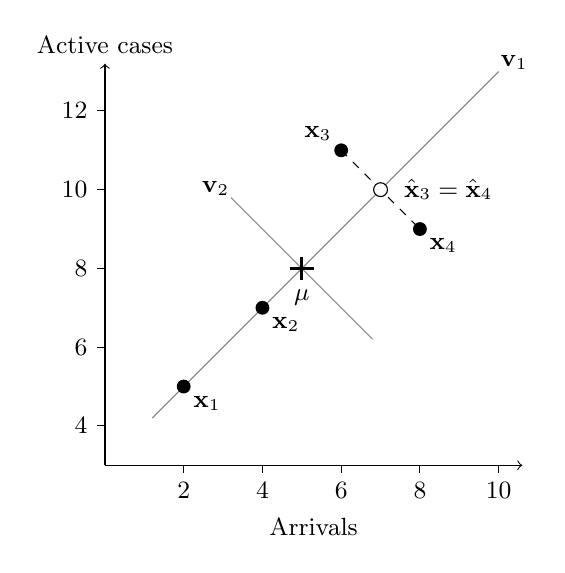
\begin{tikzpicture}[x=0.5cm, y=0.5cm, font=\small]
		% axes, the y-axis starts at 3 to save space
		\draw[->] (0, 3) -- (10.6, 3);
		\node[below=0.55cm] at (5.3, 3) {Arrivals};
		\draw[->] (0, 3) -- (0, 13.2) node[above] {Active cases};
		\foreach \x in {2, 4, 6, 8, 10}
			\draw (\x, 3) -- (\x, 2.8) node[below] {\x};
		\foreach \y in {4, 6, 8, 10, 12}
			\draw (0, \y) -- (-0.2, \y) node[left] {\y};
		% principal components as new axes through the mean
		\draw[black!45] (1.2, 4.2) -- (10, 13) node[above right=-0.1cm, text=black] {$\mathbf{v}_1$};
		\draw[black!45] (6.8, 6.2) -- (3.2, 9.8) node[above left=-0.1cm, text=black] {$\mathbf{v}_2$};
		% reconstruction errors of x_3 and x_4
		\draw[dashed] (6, 11) -- (7, 10) -- (8, 9);
		% feature vectors
		\fill (2, 5) circle (2.5pt) node[below right] {$\mathbf{x}_1$};
		\fill (4, 7) circle (2.5pt) node[below right] {$\mathbf{x}_2$};
		\fill (6, 11) circle (2.5pt) node[above left] {$\mathbf{x}_3$};
		\fill (8, 9) circle (2.5pt) node[below right] {$\mathbf{x}_4$};
		% mean and reconstruction
		\draw[very thick] (4.7, 8) -- (5.3, 8) (5, 7.7) -- (5, 8.3);
		\node[below=0.15cm] at (5, 8) {$\boldsymbol{\mu}$};
		\draw[fill=white] (7, 10) circle (2.5pt);
		\node[right] at (7.35, 10) {$\hat{\mathbf{x}}_3 = \hat{\mathbf{x}}_4$};
	\end{tikzpicture}
	\caption[PCA for two correlated features]{%
		PCA for the four feature vectors of Example~\ref{ex:prelim:pca}. The gray lines are the principal components through the mean $\boldsymbol{\mu}$ (cross). The variance along $\mathbf{v}_1$ is $\lambda_1 = 9$, along $\mathbf{v}_2$ only $\lambda_2 = 1$. Thus, the projection onto $\mathbf{v}_1$ keeps 90\% of the variance. The reconstructions of $\mathbf{x}_1$ and $\mathbf{x}_2$ are exact. $\mathbf{x}_3$ and $\mathbf{x}_4$ are both reconstructed as $(7, 10)^\top$ (empty circle), and the dashed lines are their reconstruction errors.}
	\label{fig:prelim:pca}
\end{figure}

\begin{example}
	\label{ex:prelim:pca}
	Four calendar windows are described by their number of arrivals and their number of active cases.
	\begin{itemize}
		\item The feature vectors $\mathbf{x}_1 = (2, 5)^\top$, $\mathbf{x}_2 = (4, 7)^\top$, $\mathbf{x}_3 = (6, 11)^\top$ and $\mathbf{x}_4 = (8, 9)^\top$ have the mean vector and the covariance matrix
		      \[
			      \boldsymbol{\mu} = \begin{pmatrix} 5 \\ 8 \end{pmatrix}
			      \quad\text{and}\quad
			      \Sigma = \begin{pmatrix} 5 & 4 \\ 4 & 5 \end{pmatrix}.
		      \]

		\item Both features have the same variance, so scaling does not change the principal components.

		\item $\Sigma$ has the eigenvalues $\lambda_1 = 9$ and $\lambda_2 = 1$ with the eigenvectors $\mathbf{v}_1 = (1, 1)^\top / \sqrt{2}$ and $\mathbf{v}_2 = (-1, 1)^\top / \sqrt{2}$.

		\item The first principal component explains $\mathit{evr}_X(1) = 9/10$ of the variance, since windows with many arrivals also have many active cases.

		\item The projections onto $\mathbf{v}_1$ are $-3\sqrt{2}$, $-\sqrt{2}$, $2\sqrt{2}$ and $2\sqrt{2}$.

		\item The reconstructions of $\mathbf{x}_1$ and $\mathbf{x}_2$ are exact. $\mathbf{x}_3$ and $\mathbf{x}_4$ are both reconstructed as $(7, 10)^\top$ with the squared error 2, so $\mathit{err}_X(1) = (0 + 0 + 2 + 2) / 4 = 1 = \lambda_2$ (Figure~\ref{fig:prelim:pca}).
	\end{itemize}
\end{example}

\section{Clustering}
\label{sec:prelim:clustering}
A clustering algorithm groups vectors such that vectors in the same group are similar to each other. Let $X \in \R^{m \times n}$ be a feature matrix with the rows $\mathbf{x}_1^\top, \dots, \mathbf{x}_m^\top$. A clustering of $X$ is a function $\mathit{cl} \in \Set{1, \dots, m} \to K$ that assigns each vector a cluster from a set $K$. The following three algorithms form clusters in different ways:
\begin{itemize}
	\item \emph{k-means} forms a given number of clusters around centers (Section~\ref{sec:prelim:kmeans}).
	\item A \emph{self-organizing map} arranges prototypes on a grid whose cells are the clusters (Section~\ref{sec:prelim:som}).
	\item \emph{DBSCAN} merges dense regions into clusters and marks the vectors outside them as noise (Section~\ref{sec:prelim:dbscan}).
\end{itemize}
Figure~\ref{fig:prelim:clustering} applies all three algorithms to the same vectors. Section~\ref{sec:prelim:cluster_eval} introduces metrics that evaluate the resulting clusterings.

\subsection{k-Means}
\label{sec:prelim:kmeans}
k-means searches $k$ centers such that the squared distances of the vectors to their nearest center are as small as possible.

\begin{definition}[k-Means]
	\label{def:prelim:kmeans}
	Let $X \in \R^{m \times n}$ be a feature matrix with the rows $\mathbf{x}_1^\top, \allowbreak \dots, \allowbreak \mathbf{x}_m^\top$ and $k \in \N$ with $k \le m$. A k-means clustering of $X$ consists of centers $\mathbf{c}_1, \dots, \mathbf{c}_k \in \R^n$ and a clustering $\mathit{cl} \in \Set{1, \dots, m} \to \Set{1, \dots, k}$ such that
	\begin{itemize}
		\item each vector belongs to its nearest center, i.e., $\mathit{cl}(j) \in \argmin_{1 \le l \le k} \norm{\mathbf{x}_j - \mathbf{c}_l}$ for $1 \le j \le m$, and
		\item each center is the mean of its vectors, i.e., for $1 \le l \le k$,
		      \[
			      \mathbf{c}_l = \frac{1}{\abs{J_l}} \sum_{j \in J_l} \mathbf{x}_j
			      \quad\text{with}\quad
			      J_l = \Set{j \given \mathit{cl}(j) = l} \neq \emptyset.
		      \]
	\end{itemize}
\end{definition}

k-means finds such a clustering by starting with $k$ randomly chosen vectors as centers. It then establishes both conditions alternately until the assignment does not change anymore.

\medskip
\noindent\emph{Properties:}
\begin{itemize}[beginpenalty=10000]
	\item k-means needs the number $k$ of clusters in advance.
	\item Outliers always belong to a cluster.
	\item The result depends on the initial centers.
\end{itemize}

\subsection{Self-Organizing Maps}
\label{sec:prelim:som}
A self-organizing map (SOM) is a neural network whose neurons lie on a usually two-dimensional grid. The model goes back to Kohonen~\autocite{haykin2009neural}. We call a neuron a cell of the grid. Each cell has a prototype in the feature space, and a vector belongs to the cell with the nearest prototype. During training, the cells compete for each vector, the winning cell pulls its neighbors along, and the prototypes adapt to the vector.

\begin{definition}[Self-Organizing Map]
	\label{def:prelim:som}
	Let $X \in \R^{m \times n}$ be a feature matrix with the rows $\mathbf{x}_1^\top, \dots, \mathbf{x}_m^\top$ and $G = \Set{1, \dots, p} \times \Set{1, \dots, q}$ a grid with $p, q \in \N$.
	\begin{itemize}
		\item A SOM assigns each cell $\mathbf{r} \in G$ a prototype $\mathbf{w}_{\mathbf{r}}(t) \in \R^n$ at time $t \in \N_0$.
		\item The best-matching unit (BMU) of a vector $\mathbf{x} \in \R^n$ at time $t$ is the cell $b_t(\mathbf{x}) = \argmin_{\mathbf{r} \in G} \norm{\mathbf{x} - \mathbf{w}_{\mathbf{r}}(t)}$.
		\item The initial prototypes $\mathbf{w}_{\mathbf{r}}(0)$ are, e.g., randomly chosen vectors of $X$.
		\item In each step $t = 0, 1, \dots, T - 1$, a vector $\mathbf{x}(t) \in \Set{\mathbf{x}_1, \dots, \mathbf{x}_m}$ is chosen, and all prototypes move towards it:
		      \[
			      \mathbf{w}_{\mathbf{r}}(t + 1) = \mathbf{w}_{\mathbf{r}}(t) + \eta(t) \, h_{b_t(\mathbf{x}(t)), \mathbf{r}}(t) \, \bigl(\mathbf{x}(t) - \mathbf{w}_{\mathbf{r}}(t)\bigr) \quad \text{for all } \mathbf{r} \in G.
		      \]
		\item The neighborhood function $h_{\mathbf{b}, \mathbf{r}}(t) = \exp\bigl(-\norm{\mathbf{b} - \mathbf{r}}^2 / (2 \sigma(t)^2)\bigr)$ decreases with the grid distance of the cells $\mathbf{b}$ and $\mathbf{r}$.
		\item The learning rate $\eta(t) > 0$ and the neighborhood radius $\sigma(t) > 0$ decrease monotonically in $t$.
		\item After $T$ steps, the SOM yields the clustering $\mathit{cl}(j) = b_T(\mathbf{x}_j)$ with $K = G$.
	\end{itemize}
\end{definition}

\noindent\emph{Properties:}
\begin{itemize}[beginpenalty=10000]
	\item The neighborhood function also pulls the neighbors of the BMU towards the vector. Thus, neighboring cells get similar prototypes, and vectors that are close in the feature space fall into close cells.
	\item Towards the end of the training, $\sigma(t)$ is so small that almost only the BMU adapts.
	\item The SOM forms at most $p \cdot q$ clusters.
	\item As in k-means, every vector belongs to a cluster.
	\item Similarly to k-means, the grid size must be specified in advance.
	\item Instead of the Euclidean distance, the BMU can be determined with another distance, e.g., the Manhattan, Chebyshev or cosine distance. The update of the prototypes stays the same.
\end{itemize}

\begin{figure}[tb]
	\centering
	\captionsetup[subfigure]{justification=centering}
	\definecolor{clusterA}{RGB}{0,114,178}
	\definecolor{clusterB}{RGB}{230,159,0}
	\definecolor{clusterC}{RGB}{0,158,115}
	\definecolor{clusterD}{RGB}{204,121,167}
	% markers: #1 is the style, #2 and #3 the coordinates
	\newcommand*{\mcirc}[3]{\path[#1] (#2, #3) circle (2.2pt);}
	\newcommand*{\msq}[3]{\path[#1] (#2, #3) ++(-2pt, -2pt) rectangle ++(4pt, 4pt);}
	\newcommand*{\mtri}[3]{\path[#1] (#2, #3) ++(0, 2.8pt) -- ++(-2.5pt, -4.3pt) -- ++(5pt, 0) -- cycle;}
	\newcommand*{\mdia}[3]{\path[#1] (#2, #3) ++(0, 2.9pt) -- ++(2.9pt, -2.9pt) -- ++(-2.9pt, -2.9pt) -- ++(-2.9pt, 2.9pt) -- cycle;}
	\newcommand*{\mnoise}[2]{\draw[black!55, line width=0.9pt] (#1, #2) ++(-2.4pt, -2.4pt) -- ++(4.8pt, 4.8pt) (#1, #2) ++(-2.4pt, 2.4pt) -- ++(4.8pt, -4.8pt);}
	\newcommand*{\mcenter}[2]{\filldraw[fill=black, draw=white, line width=0.7pt] (#1, #2) circle (3.2pt);}
	\tikzset{
		panel/.style={x=0.82cm, y=0.82cm, font=\small},
		fA/.style={fill=clusterA}, fB/.style={fill=clusterB}, fC/.style={fill=clusterC}, fD/.style={fill=clusterD},
		hB/.style={draw=clusterB, fill=white, line width=0.7pt}, hC/.style={draw=clusterC, fill=white, line width=0.7pt},
	}
	\newcommand*{\frameaxes}{%
		\draw[black!30] (0, 0) rectangle (5.2, 4.5);
		\node[below] at (2.6, 0) {Feature 1};
		\node[rotate=90, above] at (0, 2.25) {Feature 2};
	}
	\begin{subfigure}[t]{0.325\textwidth}
		\centering
		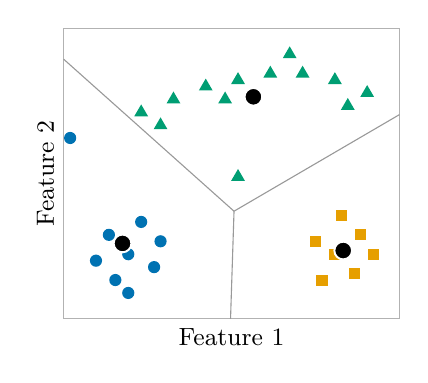
\begin{tikzpicture}[panel]
			\frameaxes
			% Voronoi cells of the three centers
			\draw[black!40] (2.638, 1.666) -- (0, 4.02) (2.638, 1.666) -- (5.2, 3.162) (2.638, 1.666) -- (2.584, 0);
			\foreach \x/\y in {1.0/1.0, 1.4/0.8, 0.7/1.3, 1.2/1.5, 0.8/0.6, 1.5/1.2, 1.0/0.4, 0.5/0.9, 0.1/2.8}
				{\mcirc{fA}{\x}{\y}}
			\foreach \x/\y in {4.2/1.0, 4.6/1.3, 4.0/0.6, 4.5/0.7, 3.9/1.2, 4.3/1.6, 4.8/1.0}
				{\msq{fB}{\x}{\y}}
			\foreach \x/\y in {1.2/3.2, 1.7/3.4, 2.2/3.6, 2.7/3.7, 3.2/3.8, 3.7/3.8, 4.2/3.7, 4.7/3.5, 1.5/3.0, 4.4/3.3, 2.5/3.4, 3.5/4.1, 2.7/2.2}
				{\mtri{fC}{\x}{\y}}
			\foreach \x/\y in {0.911/1.167, 4.329/1.057, 2.938/3.438}
				{\mcenter{\x}{\y}}
		\end{tikzpicture}
		\caption{k-means, $k = 3$}
		\label{fig:prelim:clustering_kmeans}
	\end{subfigure}%
	\hfill
	\begin{subfigure}[t]{0.325\textwidth}
		\centering
		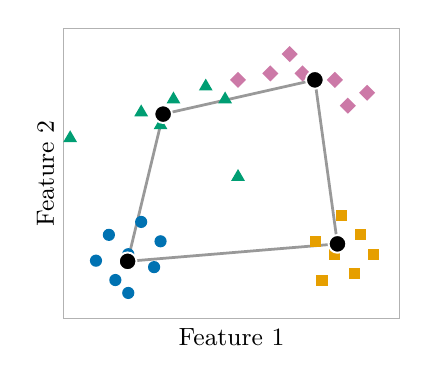
\begin{tikzpicture}[panel]
			\frameaxes
			% grid edges between the prototypes of neighboring cells
			\draw[black!40, line width=1pt] (0.99, 0.89) -- (4.24, 1.16) -- (3.89, 3.70) -- (1.54, 3.17) -- cycle;
			\foreach \x/\y in {1.0/1.0, 1.4/0.8, 0.7/1.3, 1.2/1.5, 0.8/0.6, 1.5/1.2, 1.0/0.4, 0.5/0.9}
				{\mcirc{fA}{\x}{\y}}
			\foreach \x/\y in {4.2/1.0, 4.6/1.3, 4.0/0.6, 4.5/0.7, 3.9/1.2, 4.3/1.6, 4.8/1.0}
				{\msq{fB}{\x}{\y}}
			\foreach \x/\y in {1.2/3.2, 1.7/3.4, 2.2/3.6, 1.5/3.0, 2.5/3.4, 2.7/2.2, 0.1/2.8}
				{\mtri{fC}{\x}{\y}}
			\foreach \x/\y in {2.7/3.7, 3.2/3.8, 3.7/3.8, 4.2/3.7, 4.7/3.5, 4.4/3.3, 3.5/4.1}
				{\mdia{fD}{\x}{\y}}
			\foreach \x/\y in {0.99/0.89, 4.24/1.16, 1.54/3.17, 3.89/3.70}
				{\mcenter{\x}{\y}}
		\end{tikzpicture}
		\caption{SOM, $2 \times 2$ grid}
		\label{fig:prelim:clustering_som}
	\end{subfigure}%
	\hfill
	\begin{subfigure}[t]{0.325\textwidth}
		\centering
		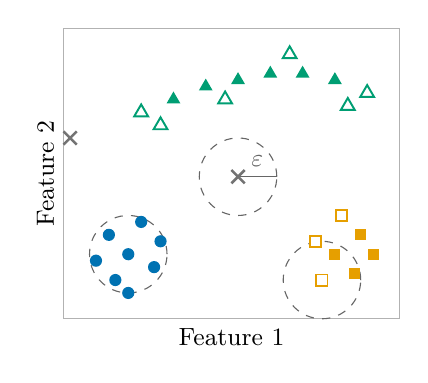
\begin{tikzpicture}[panel]
			\frameaxes
			% epsilon neighborhoods of a core point, a border point and a noise point
			\draw[dashed, black!60] (1.0, 1.0) circle (0.6) (4.0, 0.6) circle (0.6) (2.7, 2.2) circle (0.6);
			\draw[black!60] (2.7, 2.2) -- node[above] {$\varepsilon$} (3.3, 2.2);
			\foreach \x/\y in {1.0/1.0, 1.4/0.8, 0.7/1.3, 1.2/1.5, 0.8/0.6, 1.5/1.2, 1.0/0.4, 0.5/0.9}
				{\mcirc{fA}{\x}{\y}}
			\foreach \x/\y in {4.2/1.0, 4.6/1.3, 4.5/0.7, 4.8/1.0}
				{\msq{fB}{\x}{\y}}
			\foreach \x/\y in {4.0/0.6, 3.9/1.2, 4.3/1.6}
				{\msq{hB}{\x}{\y}}
			\foreach \x/\y in {1.7/3.4, 2.2/3.6, 2.7/3.7, 3.2/3.8, 3.7/3.8, 4.2/3.7}
				{\mtri{fC}{\x}{\y}}
			\foreach \x/\y in {1.2/3.2, 4.7/3.5, 1.5/3.0, 4.4/3.3, 2.5/3.4, 3.5/4.1}
				{\mtri{hC}{\x}{\y}}
			\mnoise{2.7}{2.2}
			\mnoise{0.1}{2.8}
		\end{tikzpicture}
		\caption{DBSCAN, $\varepsilon = 0.6$, $\mathit{minPts} = 4$}
		\label{fig:prelim:clustering_dbscan}
	\end{subfigure}
	\caption[Three clustering algorithms in comparison]{%
		The three clustering algorithms of Example~\ref{ex:prelim:clustering} on the same 29 vectors with three groups and two outliers. Color and shape of a symbol show its cluster, and black dots are the centers or prototypes.
		\subref{fig:prelim:clustering_kmeans}~k-means divides the plane into convex cells (gray lines) and also assigns the outliers to a cluster.
		\subref{fig:prelim:clustering_som}~The gray line connects the prototypes of neighboring cells: $(1, 1)$ bottom left, $(1, 2)$ bottom right, $(2, 2)$ top right and $(2, 1)$ top left. The elongated group is split into the cells $(2, 1)$ and $(2, 2)$.
		\subref{fig:prelim:clustering_dbscan}~DBSCAN detects the outliers as noise (gray crosses). Filled symbols are core points and empty symbols border points. The dashed circles show the $\varepsilon$-neighborhood of a core point, a border point and an outlier.}
	\label{fig:prelim:clustering}
\end{figure}

\subsection{DBSCAN}
\label{sec:prelim:dbscan}
DBSCAN forms clusters from regions in which vectors lie densely (\textcite{ester1996density}). A region is dense if at least $\mathit{minPts}$ vectors lie within the radius $\varepsilon$ of a vector. Vectors in sparse regions belong to no cluster and count as noise.

\begin{definition}[DBSCAN]
	\label{def:prelim:dbscan}
	Let $X \in \R^{m \times n}$ be a feature matrix with the rows $\mathbf{x}_1^\top, \dots, \mathbf{x}_m^\top$, $I = \Set{1, \dots, m}$, $\varepsilon \in \R$ with $\varepsilon > 0$ and $\mathit{minPts} \in \N$.
	\begin{itemize}
		\item $N_\varepsilon(j) = \Set{l \in I \given \norm{\mathbf{x}_j - \mathbf{x}_l} \le \varepsilon}$ is the $\varepsilon$-neighborhood of $j \in I$. It contains $j$ itself.
		\item $j \in I$ is a core point if $\abs{N_\varepsilon(j)} \ge \mathit{minPts}$.
		\item $l \in I$ is directly density-reachable from $j \in I$ if $j$ is a core point and $l \in N_\varepsilon(j)$. $l$ is density-reachable from $j$ if there are $i_1, \dots, i_r \in I$ with $i_1 = j$ and $i_r = l$ such that $i_{h+1}$ is directly density-reachable from $i_h$ for $1 \le h < r$.
		\item A cluster is a non-empty set $C \subseteq I$ that is maximal and connected. Maximal means that $l \in C$ if $j \in C$ and $l$ is density-reachable from $j$. Connected means that for all $j, l \in C$, there is an $i \in I$ from which both $j$ and $l$ are density-reachable.
		\item The points of a cluster that are not core points are border points. Points that belong to no cluster are noise.
		\item For the clusters $C_1, \dots, C_k$, the clustering is $\mathit{cl}(j) = l$ for $j \in C_l$ and $\mathit{cl}(j) = \mathit{noise}$ if $j$ is noise. Thus, $K = \Set{1, \dots, k, \mathit{noise}}$.
	\end{itemize}
\end{definition}

\noindent\emph{Properties:}
\begin{itemize}[beginpenalty=10000]
	\item Unlike in k-means and the SOM, the number of clusters follows from the data.
	\item Any distance can replace the Euclidean distance in the $\varepsilon$-neighborhood~\autocite{ester1996density}, e.g., the Manhattan, Chebyshev or cosine distance.
	\item A common approach to choose $\varepsilon$ is using the first valley area of the sorted $k$-dist graph with $k = \mathit{minPts}$. This graph shows the distance of each point to its $k$-th nearest neighbor in descending order.
\end{itemize}

\begin{example}
	\label{ex:prelim:clustering}
	Figure~\ref{fig:prelim:clustering} shows 29 vectors in $\R^2$: three groups, one of them elongated, and two outliers.
	\begin{itemize}
		\item k-means with $k = 3$ finds the three groups, but also assigns both outliers to a cluster.

		\item The SOM with a $2 \times 2$ grid has four cells for three groups. Therefore, it splits the elongated group into two neighboring cells.

		\item DBSCAN with $\varepsilon = 0.6$ and $\mathit{minPts} = 4$ finds exactly the three groups and detects both outliers as noise.
	\end{itemize}
\end{example}

\subsection{Clustering Evaluation}
\label{sec:prelim:cluster_eval}
The true groups of the vectors are unknown. Thus, a clustering can only be evaluated with the vectors themselves, e.g., by how compact and how well separated its clusters are. We use five such metrics. The silhouette and the Cali\'nski--Harabasz index evaluate the clusterings of all three algorithms. The quantization error and the occupancy entropy evaluate SOMs, and DBCV evaluates DBSCAN. For SOMs and DBSCAN, the silhouette, the quantization error and DBCV use the same distance as the clustering. The Cali\'nski--Harabasz index always uses the Euclidean distance.

\medskip
\noindent\emph{Clusters:}
\begin{itemize}[beginpenalty=10000]
	\item The clusters of a clustering $\mathit{cl}$ of a feature matrix $X \in \R^{m \times n}$ are the non-empty sets $\Set{j \given \mathit{cl}(j) = \kappa}$ with $\kappa \in K \setminus \Set{\mathit{noise}}$. We number them $C_1, \dots, C_k$.
	\item Noise belongs to no cluster, and $I' = C_1 \cup \dots \cup C_k$ contains the $m' = \abs{I'}$ clustered vectors.
\end{itemize}

The silhouette compares the distance of a vector to its own cluster with its distance to the nearest other cluster~\autocite{rousseeuw1987silhouettes}. The Cali\'nski--Harabasz index compares the dispersion between the clusters with the dispersion within them~\autocite{calinski1974dendrite}.

\begin{definition}[Silhouette]
	\label{def:prelim:silhouette}
	Let $\mathit{cl}$ be a clustering of a feature matrix $X \in \R^{m \times n}$ with $k \ge 2$ clusters and $m' > k$. For $j \in C_l$, let
	\[
		a(j) = \frac{1}{\abs{C_l} - 1} \sum_{i \in C_l \setminus \Set{j}} \norm{\mathbf{x}_j - \mathbf{x}_i}
		\quad\text{and}\quad
		b(j) = \min_{l' \neq l} \frac{1}{\abs{C_{l'}}} \sum_{i \in C_{l'}} \norm{\mathbf{x}_j - \mathbf{x}_i}
	\]
	be the mean distances of $\mathbf{x}_j$ to the other vectors of its cluster and to the vectors of the nearest other cluster.
	\begin{itemize}
		\item $s(j) = (b(j) - a(j)) / \max\Set{a(j), b(j)}$ is the silhouette of $j$, and $s(j) = 0$ if $\abs{C_l} = 1$.
		\item $\mathit{sil}(\mathit{cl}) = \frac{1}{m'} \sum_{j \in I'} s(j)$ is the silhouette of $\mathit{cl}$.
	\end{itemize}
\end{definition}

\begin{definition}[Cali\'nski--Harabasz Index]
	\label{def:prelim:ch}
	Let $\mathit{cl}$ be a clustering of a feature matrix $X \in \R^{m \times n}$ with $k \ge 2$ clusters and $m' > k$. Let $\boldsymbol{\mu}'$ be the mean of the clustered vectors $\mathbf{x}_j$ with $j \in I'$, and $\mathbf{c}_l$ the mean of the vectors of $C_l$.
	\begin{itemize}
		\item $D_b = \sum_{l=1}^{k} \abs{C_l} \norm{\mathbf{c}_l - \boldsymbol{\mu}'}^2$ is the dispersion between the clusters.
		\item $D_w = \sum_{l=1}^{k} \sum_{j \in C_l} \norm{\mathbf{x}_j - \mathbf{c}_l}^2$ is the dispersion within the clusters.
		\item For $D_w > 0$, the Cali\'nski--Harabasz index of $\mathit{cl}$ is
		      \[
			      \mathit{ch}(\mathit{cl}) = \frac{D_b / (k - 1)}{D_w / (m' - k)}.
		      \]
	\end{itemize}
\end{definition}

\noindent\emph{Properties:}
\begin{itemize}[beginpenalty=10000]
	\item $s(j) > 0$ if $\mathbf{x}_j$ lies closer to its own cluster than to the nearest other one. A silhouette close to 1 shows that $\mathbf{x}_j$ lies well within its cluster, and one close to 0 that it lies between two clusters.
	\item $-1 \le \mathit{sil}(\mathit{cl}) \le 1$, and \textcite{rousseeuw1987silhouettes} uses the mean silhouette to choose the number of clusters.
	\item $\mathit{ch}(\mathit{cl})$ is large if the clusters are compact and lie far apart. It has no upper bound and depends on the scale of the features. Thus, it only compares clusterings of the same vectors.
\end{itemize}

For SOMs, we also measure how closely the prototypes fit the vectors and how evenly the vectors spread over the grid. \textcite{berti2025ocel} use both measures for the grid of their execution states.

\begin{definition}[Quantization Error, Occupancy Entropy]
	\label{def:prelim:som_eval}
	Let $\mathit{cl}$ be the clustering of a SOM after $T$ steps (Definition~\ref{def:prelim:som}) with the prototypes $\mathbf{w}_{\mathbf{r}} = \mathbf{w}_{\mathbf{r}}(T)$ on a grid $G$ with $p \cdot q \ge 2$ cells.
	\begin{itemize}
		\item $\mathit{qe}(\mathit{cl}) = \frac{1}{m} \sum_{j=1}^{m} \norm{\mathbf{x}_j - \mathbf{w}_{\mathit{cl}(j)}}$ is the quantization error, i.e., the mean distance of the vectors to the prototypes of their cells.
		\item $\mathit{occ}(\mathbf{r}) = \abs{\Set{j \given \mathit{cl}(j) = \mathbf{r}}} / m$ is the occupancy of a cell $\mathbf{r} \in G$, i.e., the share of the vectors in $\mathbf{r}$.
		\item The occupancy entropy of $\mathit{cl}$ is
		      \[
			      \mathit{ent}(\mathit{cl}) = -\frac{1}{\log(p \cdot q)} \sum_{\mathbf{r} \in G,\, \mathit{occ}(\mathbf{r}) > 0} \mathit{occ}(\mathbf{r}) \log \mathit{occ}(\mathbf{r}).
		      \]
	\end{itemize}
\end{definition}

\noindent\emph{Properties:}
\begin{itemize}[beginpenalty=10000]
	\item A small quantization error means that the prototypes lie close to their vectors.
	\item The occupancy entropy is 0 if all vectors lie in one cell and 1 if all cells hold equally many vectors.
\end{itemize}

DBCV, the density-based clustering validation, compares the density within the clusters with the density between them (\textcite{moulavi2014density}). In a good clustering, even the sparsest region inside a cluster is denser than the region that separates it from the other clusters.

\begin{definition}[Density-Based Clustering Validation]
	\label{def:prelim:dbcv}
	Let $\mathit{cl}$ be a DBSCAN clustering of a feature matrix $X \in \R^{m \times n}$ with $k \ge 2$ clusters.
	\begin{itemize}
		\item The density sparseness $\mathit{dsc}(C_l)$ is the largest gap that the vectors of $C_l$ have to bridge to connect each other, i.e., the sparsest region inside $C_l$.
		\item The density separation $\mathit{sep}(C_l)$ is the smallest gap between $C_l$ and another cluster, i.e., the densest region between them.
		\item The validity of $C_l$ is
		      \[
			      v(C_l) = \frac{\mathit{sep}(C_l) - \mathit{dsc}(C_l)}{\max\Set{\mathit{sep}(C_l), \mathit{dsc}(C_l)}}.
		      \]
		\item $\mathit{dbcv}(\mathit{cl}) = \sum_{l=1}^{k} \frac{\abs{C_l}}{m} \, v(C_l)$ is the DBCV of $\mathit{cl}$, where $m$ also counts the noise.
	\end{itemize}
\end{definition}

\noindent\emph{Properties:}
\begin{itemize}[beginpenalty=10000]
	\item Both gaps are taken from a minimum spanning tree of each cluster, whose edge weights grow in sparse regions. The tree also captures the shape of the cluster, so DBCV evaluates clusters of arbitrary shape~\autocite{moulavi2014density}.
	\item $v(C_l) > 0$ if $C_l$ is denser inside than towards the nearest other cluster. The DBCV lies between $-1$ and $1$~\autocite{moulavi2014density}.
	\item Noise lowers the DBCV, since it counts in $m$ but belongs to no cluster~\autocite{moulavi2014density}.
\end{itemize}

\begin{table}[htb]
	\centering
	\caption[Evaluation of the example clusterings]{%
		Metrics of the three clusterings in Figure~\ref{fig:prelim:clustering}.}
	\label{tab:prelim:cluster_eval}
	\begin{tabular}{@{}lrrrrr@{}}
		\toprule
		Clustering                                         & $\mathit{sil}$ & $\mathit{ch}$ & $\mathit{qe}$ & $\mathit{ent}$ & $\mathit{dbcv}$ \\
		\midrule
		k-means, $k = 3$                                   & 0.573          & 45.4          & --            & --             & --              \\
		SOM, $2 \times 2$ grid                             & 0.585          & 65.5          & 0.575         & 0.999          & --              \\
		DBSCAN, $\varepsilon = 0.6$, $\mathit{minPts} = 4$ & 0.627          & 52.7          & --            & --             & 0.684           \\
		\bottomrule
	\end{tabular}
\end{table}

\begin{example}
	\label{ex:prelim:cluster_eval}
	Table~\ref{tab:prelim:cluster_eval} evaluates the clusterings of Example~\ref{ex:prelim:clustering}.
	\begin{itemize}[beginpenalty=10000]
		\item DBSCAN has the highest silhouette, since it leaves out the two outliers. In k-means, the outlier $(2.7, 2.2)$ only has the silhouette 0.125.

		\item The elongated group has the lowest mean silhouette in all three clusterings.

		\item The SOM has the highest Cali\'nski--Harabasz index, although it splits the elongated group.

		\item The SOM uses its four cells almost evenly with 8, 7, 7 and 7 vectors, so its occupancy entropy is close to 1. Its quantization error is the mean distance of the vectors to the black dots in Figure~\ref{fig:prelim:clustering_som}.

		\item DBSCAN has the DBCV 0.684. Since the two noise vectors count in $m = 29$, the DBCV is at most $27/29 \approx 0.931$ here.
	\end{itemize}
\end{example}
